\chapter{Design}
\section{Actors}

There are three main actors: 
\begin{itemize}
	\item Reviewer (User)
	\item Company Manager (Super User)
	\item Administrator 
	The \emph{Reviewer} is the end-user of the application, who is able to search for \emph{videogames}, review them, comment on other users' reviews, etc 
	The \emph{Company Manager} is an entity that represents the owner 
\end{itemize}
\section{Requirements}
\subsection{Functional Requirements}
\subsubsection{Handled by MongoDB}
\begin{itemize}
	\item Average review score per game producer 
	\item Most active Users (looking at the number of posted reviews)
	\item Most discussed reviews 
	\item Most popular games in the latest week/month/year 
\end{itemize}
\subsubsection{Handled by Neo4j}
\begin{itemize}
	\item New friend recommendations 
	\item Videogame recommendations 
	\item identify the most influential users 
\end{itemize}
\subsection{Non-Functional Requirements}
\section{Use Case Diagram}
\begin{figure}[t]
	\centering
	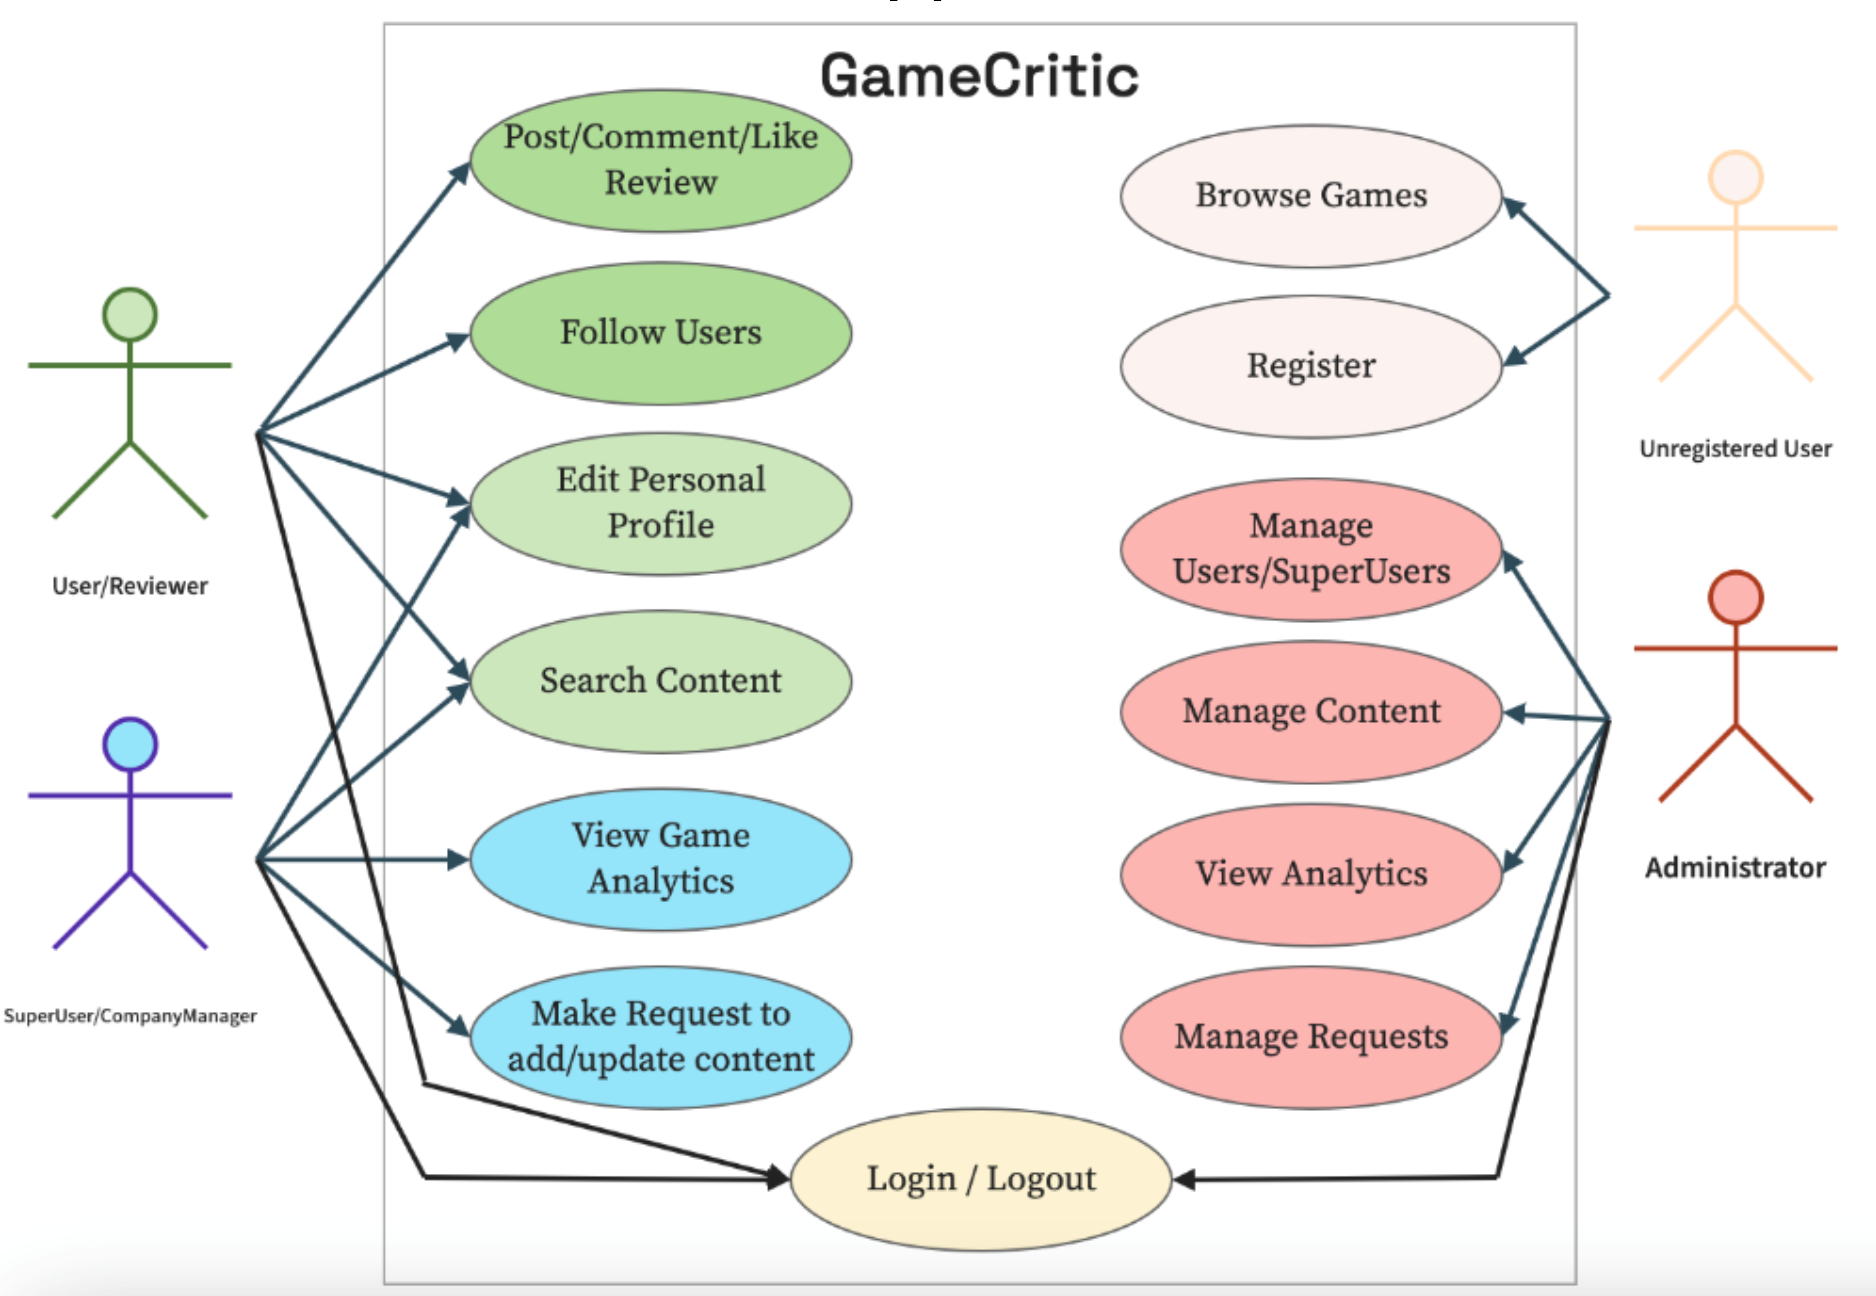
\includegraphics[width=1\textwidth]{chapter3/img/usecase.png}
	\caption{Actors and main supported functionalities}
	\label{fig:usecase}
\end{figure}
\section{UML Class Diagram}
\begin{figure}[t]
	\centering
	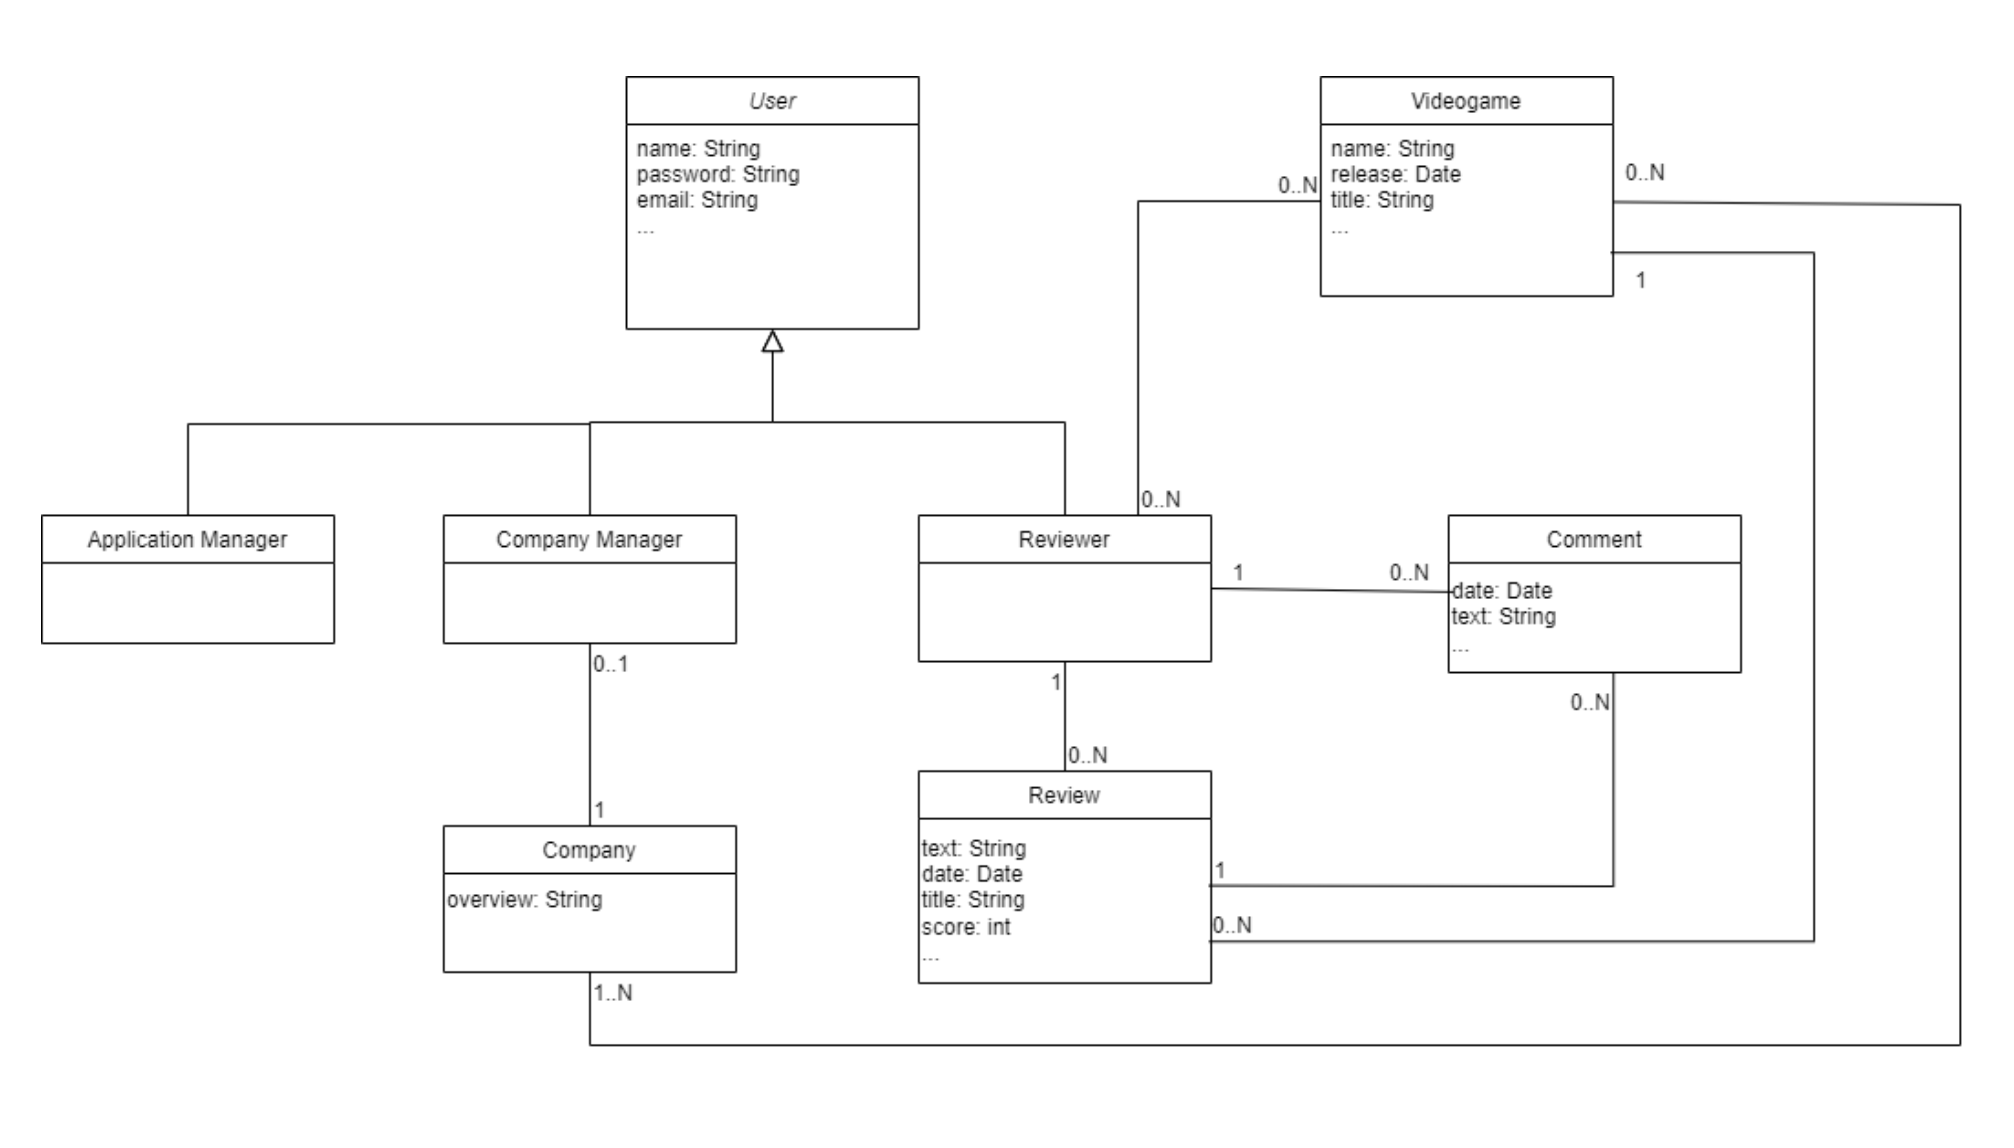
\includegraphics[width=1\textwidth]{chapter3/img/uml.png}
	\caption{UML Class Diagram}
	\label{fig:uml}
\end{figure}
\section{Data Models and Implementation}
\subsection{Document DB Collections}
\begin{itemize}
	\item Videogames 
	\item Users
	\item Reviews 
	\item Comments 
	\item userImages 
\end{itemize}
\subsection{Document DB Relationships}
\subsection{Document DB Examples}
\begin{python}
    {
	"Name": "(Almost) Total Mayhem",
	"Released": "January 14th, 2011 on Xbox 360",
	"Publishers": "Peanut Gallery",
	"Developers": "Peanut Gallery",
	"Genre": "Action",
	"Perspective": "Side view",
	"Gameplay": "Platform",
	"Setting": "Fantasy",
	"Media Type": "Download",
	"Multiplayer Options": "Same/Split-Screen",
	"Number of Offline Players": "1-2 Players",
	"Description": "description",
	"user_review": 6.0,
	"reviews": [
	{
		"score": 8,
		"quote": "stunning graphhcs!",
		"author": "Yusoreqa",
		"date": "2023-10-30",
		"source": "random",
		"comments": [
		{
			"author": "Hojosu",
			"quote": "I see that Yusoreqa agrees with me.",
			"date": "2023-12-06"
		}
		]
	}
	]
}
\end{python}
\subsection{Graph DB - Neo4j}
\begin{figure}[t]
	\centering
	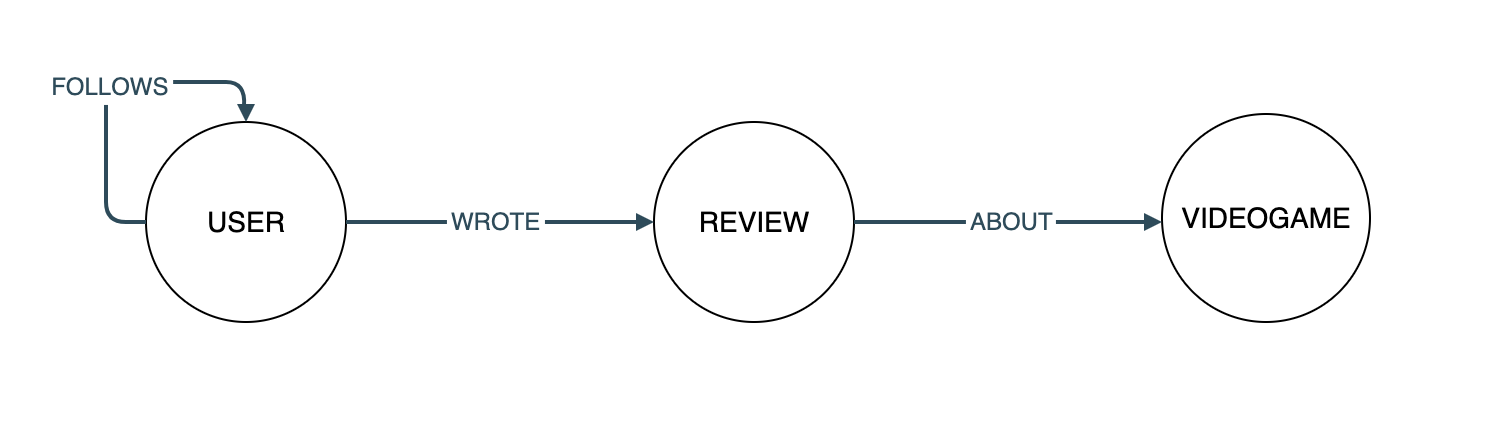
\includegraphics[width=1\textwidth]{chapter3/img/graph.png}
	\caption{Entities handled by \emph{GraphDB} and their relationships}
	\label{fig:graph}
\end{figure}
We handled the following entities via GraphDB (figure \ref{fig:graph}) :
\begin{itemize}
	\item Users 
	\item Videogames 
	\item Reviews
\end{itemize}
\section{Distributed Database Design}
Eventual consistency is sufficient, enforcing strong consistency would be too costly. 
\subsection{Replicas}
\begin{figure}[t]
	\centering
	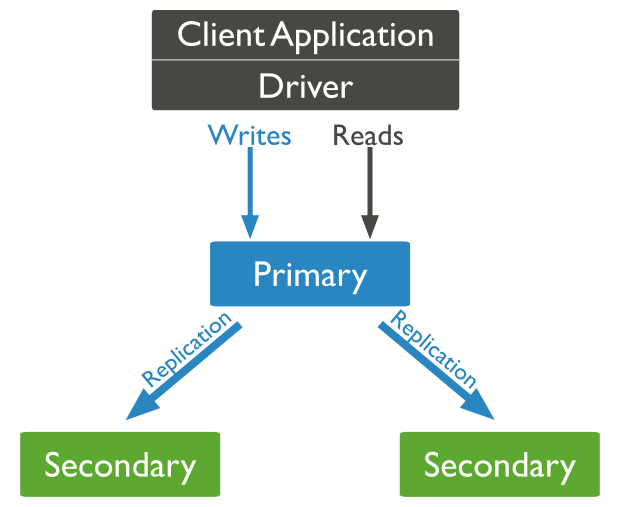
\includegraphics[width=0.5\textwidth]{chapter3/img/replica.png}
	\caption{Replica Set}
	\label{fig:replica}
\end{figure}
We were given the chance to exploit a cluster of three nodes for the project. We deployed one \emph{MongoDB replica} for each node (replicas were not implemented for \emph{Neo4j} since to do so we would have needed the \emph{Enterprise edition}). 
The \emph{primary} is the only member in the replica set that receives write operations (figure \ref{fig:replica}). MongoDB applies write operations on the primary and then records the operations on the primary's \emph{oplog}. \emph{Secondary} members replicate this log and apply the operations to their data sets.
\subsubsection{Write Concern}

\subsection{Sharding}
\emph{mongos} instances will pass the \emph{write concern} on to the shards
\subsection{Handling inter-databases consistency}
\begin{figure}[t]
	\centering
	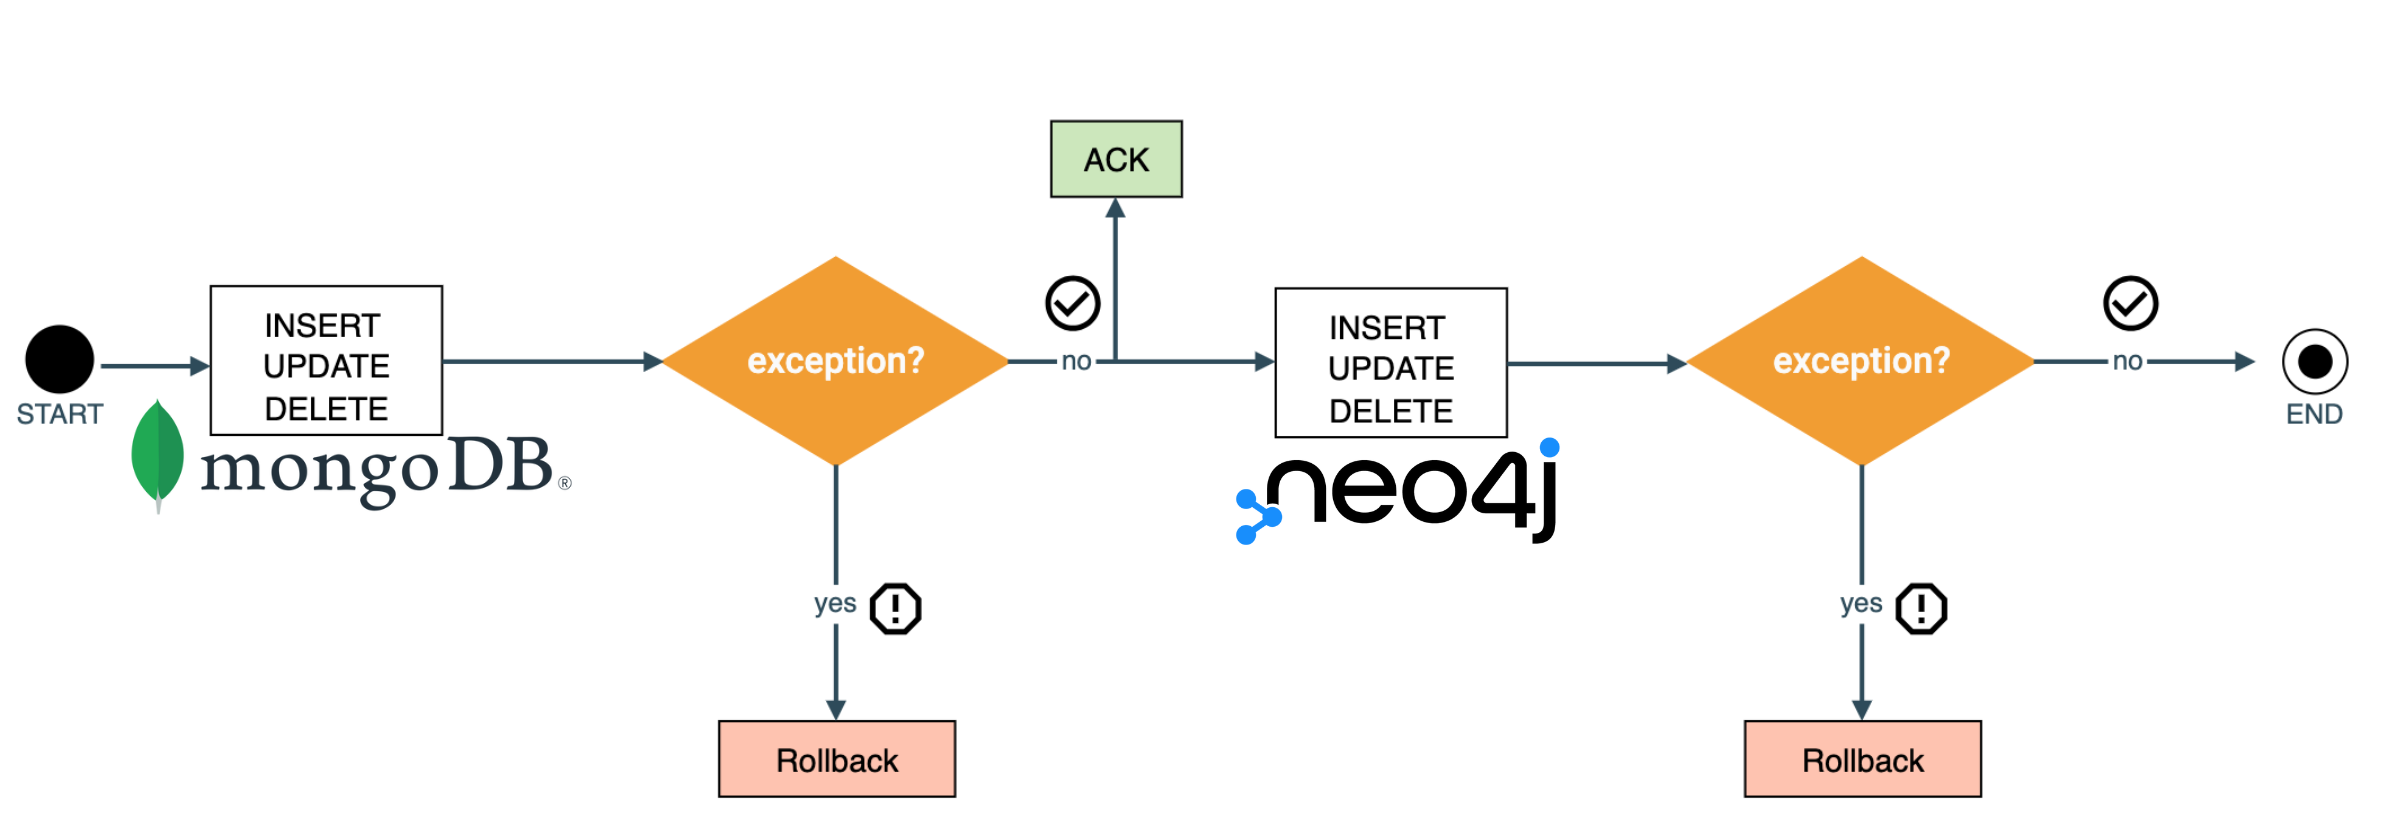
\includegraphics[width=1\textwidth]{chapter3/img/rollback.png}
	\caption{Handling consistency between \emph{MongoDB} and \emph{Neo4j}}
	\label{fig:rb}
\end{figure}
Having to deal with two different architectures (\emph{DocumentDB} and \emph{GraphDB}), we need to face the problem of redundancy and handle the consistency of data that are stored within both databases. 
Any rollback triggered by a failure of an insert, an update or a delete operation, can lead to inconsistencies. 
To address this problem, whenever a write operation  is performed successfully on \emph{MongoDB}, an ACK (\emph{acknowledgement}) is sent to the user. Data on \emph{GraphDB} will be eventually consistent: if any exception occurs when the updates over data on \emph{Neo4j} are attempted, than a rollback operation will be executed in order to bring back both the databases in a consistent state (just as shown in figure \ref{fig:rb}).
\subsubsection{Eventual Consistency}
Eventual consistency is dealt with by exploiting the \emph{asynchronous execution support} in \emph{Spring} and the \emph{@Async} annotation.
The caller will not have to wait for the complete execution of the called method: annotating a method of a bean with \emph{@Async} will make it execute in a separate thread. 